\chapter{Introduktionsopgaver}
Som kort beskrevet i Introduktionen begyndte vi dette projekt med at lave en række opgaver, både håndregningsopgaver og en del programmeringsopgaver.

\section{Håndregningsopgaver}
Vores besvarelser af håndregningsopgaverne omhandlende bit- og hexadecimalmanipulation kan ses på figur \ref{fig:Ex1.1}, figur \ref{fig:Ex2.1}, figur \ref{fig:Ex3.1} og figur \ref{fig:Ex4.4}.\\ \\ \\ \\

\begin{figure}[h!]
\centering
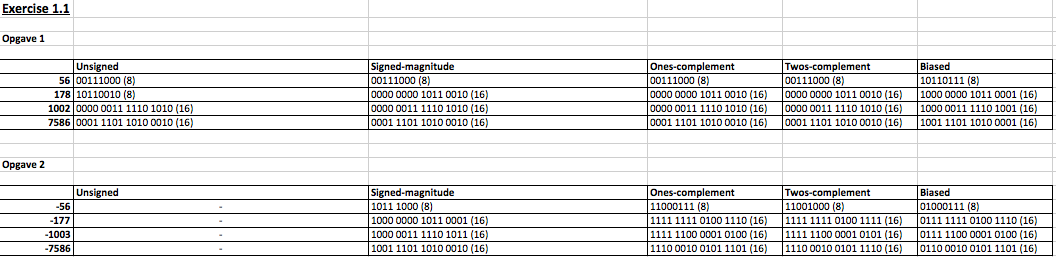
\includegraphics[scale=0.4]{figs/Ex1.png}
\caption{Vores besvarelse af Exercise 1.1}
\label{fig:Ex1.1}
\end{figure}

\begin{figure}[h!]
\centering
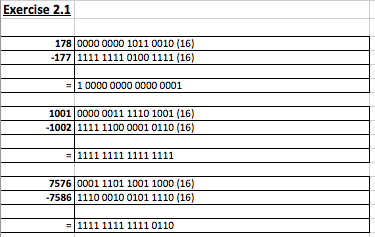
\includegraphics[scale=0.6]{figs/Ex2.png}
\caption{Vores besvarelse af Exercise 2.1}
\label{fig:Ex2.1}
\end{figure}

\begin{figure}[h!]
\centering
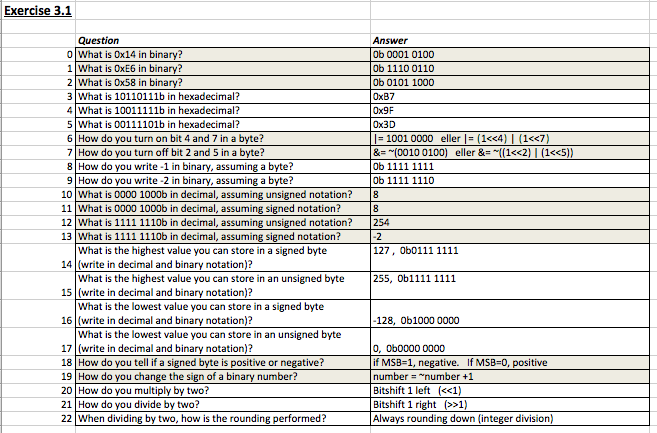
\includegraphics[scale=0.6]{figs/Ex3.png}
\caption{Vores besvarelse af Exercise 3.1}
\label{fig:Ex3.1}
\end{figure}

\begin{figure}[h!]
\centering
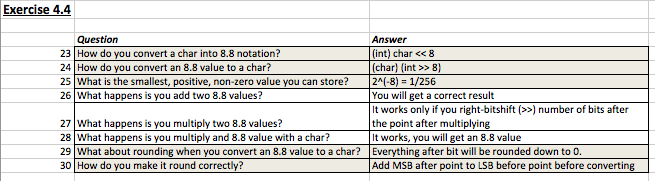
\includegraphics[scale=0.6]{figs/Ex4.png}
\caption{Vores besvarelse af Exercise 4.4}
\label{fig:Ex4.4}
\end{figure}

\newpage

\section{Programmeringsopgaver}
En del af de programmer vi skrev under introforløbet endte vi med at bruge i ReflexBall-spillet i modificerede versioner. Disse inkluderer \nameref{ansi}, \nameref{charset}, \nameref{buttons}, \nameref{LED}, \nameref{lut}, \nameref{math} og \nameref{time} og kan ses i Appendikset \textbf{\nameref{C kode}} i deres modificerede versioner. I Appendikset \textbf{\nameref{C kode}} er der fjernet noget af det oprindelige kode i \nameref{ansi} og i \nameref{time}, hvilket skyldes at vi ikke brugte de givne funktioner i implementeringen af ReflexBall. Disse fjernede dele af \textbf{ansi.c} og \textbf{time.c} kan ses nedenfor.
\newpage

\section{ansi}
\label{ansigammel}

\underline{ansi.c}
\begin{lstlisting}
void drawBanner(unsigned char x1, unsigned char y1, unsigned char left, unsigned char right, char* title) {
	gotoxy(x1+1,y1);
	printf("%c",left);
	reverse(1);
	printf("  %s  ",title);
	reverse(0);
	printf("%c",right);
}

void window(unsigned char x1, unsigned char y1, unsigned char x2, unsigned char y2, char* title, char style) {
	char* bannerTitle = title;
	unsigned char leftTop, rightTop, leftBot, rightBot, verSide, horSide, leftCross, rightCross;

	if (style) {
		leftTop = 201;
		rightTop = 187;
		leftBot = 200;
		rightBot = 188;
		verSide = 186;
		horSide = 205;
		leftCross = 185;
		rightCross = 204;
	} else {
		leftTop = 218;
		rightTop = 191;
		leftBot = 192;
		rightBot = 217;
		verSide = 179;
		horSide = 196;
		leftCross = 180;
		rightCross = 195;
	}
	
	drawTopBot(x1,y1,x2-x1-1,leftTop,rightTop,horSide);
	drawSides(x1,y1,x2,y2,verSide);
	drawTopBot(x1,y2,x2-x1-1,leftBot,rightBot,horSide);
	
	if (strlen(title) >  x2-x1-7)
		bannerTitle = "Err";
	drawBanner(x1,y1,leftCross,rightCross,bannerTitle);

	gotoxy(x1+2,y1+2);

	saveCursor();
}

void printWindow(char* string) {
	int position = 0;
	getSavedCursor();
	while(*string != '\0') {
		if (*string == '\n') {
			moveCursor(DOWN,1);
			moveCursor(BACK,position);
			position = 0;
		} else {
			printf("%c",*string);
			position++;
		}
		string++;
	}
	saveCursor();
}
\end{lstlisting}

\section{time}
\label{timegammel}

\underline{time.c}
\begin{lstlisting}

volatile unsigned char newTime = 0;
volatile time_t time;

void resetTime() {
	time.hour = 0;
	time.min = 0;
	time.sec = 0;
	time.cs = 0;
	T0H = 0; // Reset timer value
	T0L = 1;
}

void printTime(unsigned splittime) {
	if (splittime != 3)
		gotoxy(32,7+splittime);
	else
		gotoxy(32,7);
	printf("%01d:%02d:%02d.",time.hour,time.min,time.sec);
	if (splittime)
		printf("%02d",time.cs);
	else
		printf("--");
}

#pragma interrupt
void timer0int() {
	time.cs++;

	if (time.cs == 100) {
		time.cs = 0;
		time.sec++;
		newTime = 1;
		if (time.sec == 60) {
			time.sec = 0;
			time.min++;
			if (time.min == 60) {
				time.min = 0;
				time.hour++; // To the infinity!!
			}
		}
	}
}

void initWindow() {
	color(2,4);
	clrscr();
	window(10,5,45,11,"Stop watch",1);
	printWindow("Time since start:   0:00:00.--\n");
	printWindow("Split time 1:       -:--:--.--\n");
	printWindow("Split time 2:       -:--:--.--\n");
}

void initTimers() {
	DI(); // Disable interrupt
	
	T0CTL = 0; // TEN - disable timer
	T0CTL |= PRE4; // PRES - Prescaler
	T0CTL |= (1 << 0); // TMODE - continuous mode

	T0H = 0;
	T0L = 1;
	
	T0RH = 46080 >> 8; // Interrupt every 10ms
	T0RL = 46080 & 0xFF;

	SET_VECTOR(TIMER0, timer0int); // Enter the timer0int function at each interrupt
	
	// Set timer0 priority to high
	IRQ0ENH |= PRIORITY_TIMER0;
	IRQ0ENL |= PRIORITY_TIMER0;
	
	resetTime();

	//T0CTL |= (1 << 7); // TEN - enable timer

	EI(); // Enable interrupt
}
\end{lstlisting}
\newpage